\documentclass{article}

\usepackage[margin=1in]{geometry}
\usepackage{amsmath}
\usepackage{graphicx}
\usepackage{subfig}
\usepackage{tikz}

\author{Damien Prieur}
\title{Assignment 3 \\ CS 435}
\date{}

\begin{document}

\maketitle

\section{Theory Questions}

\begin{enumerate}
\item Given the following image
    $\begin{bmatrix}
    1 & 2\\
    3 & 4\\
    \end{bmatrix}$
\begin{enumerate}
\item Draw a fully connect graph representation of this image.
For pixel $a$, let $a_i$ be its value/intensity, and $(a_x,a_y )$ be its location.
We can then compute the similarity/weight between pixels a and b as:
$$w(a,b)=e^{-((a_i-b_i )^2+(a_x-b_x )^2+(a_y-b_y )^2 ) }$$

In addition, consider a pixel not to be connected to itself (weight=0).

\begin{tikzpicture}
\begin{scope}[every node/.style={circle,draw}]
    \node (ul) at (0,2){1};
    \node (ur) at (2,2){2};
    \node (ll) at (0,0){3};
    \node (lr) at (2,0){4};
\end{scope}

    \path [<->] (ul) edge node[above]{$e^{-(1+1)}$} (ur);
    \path [<->] (ul) edge node[left]{$e^{-(4 + 1)}$} (ll);
    \path [<->] (ul) edge node[sloped, above]{$e^{-(9 + 1 + 1)}$} (lr);

    \path [<->] (ur) edge[out = 0, in = -90, looseness=3.5] node[sloped, below]{$e^{-(1 + 1 + 1)}$} (ll);
    \path [<->] (ur) edge node[right]{$e^{-(4 + 1)}$} (lr);

    \path [<->] (ll) edge node[below]{$e^{-(1 + 1)}$} (lr);

\end{tikzpicture}
\begin{tikzpicture}
\begin{scope}[every node/.style={circle,draw}]
    \node (ul) at (0,2){1};
    \node (ur) at (2,2){2};
    \node (ll) at (0,0){3};
    \node (lr) at (2,0){4};
\end{scope}

    \path [<->] (ul) edge node[above]{$e^{-2}$} (ur);
    \path [<->] (ul) edge node[left]{$e^{-5}$} (ll);
    \path [<->] (ul) edge node[sloped, above]{$e^{-11}$} (lr);

    \path [<->] (ur) edge[out = 0, in = -90, looseness=3.5] node[sloped, below]{$e^{-3}$} (ll);
    \path [<->] (ur) edge node[right]{$e^{-5}$} (lr);

    \path [<->] (ll) edge node[below]{$e^{-2}$} (lr);

\end{tikzpicture}
\newline

\item Find the minimum graph cut using the matrix formulation way shown in class.
In Matlab you may use the svd function to do eigen-decomposition on a matrix.
You’ll likely need to read its documentation to understand how to the inputs and outputs work.
Show the computations needed to set up your matrix for eigen-decomposition and what the chosen eigenvalue/vector pair is.
Finally draw your new (cut) graph.
\newline
\newline
Computing our adjacency matrix we get:
$$W = \begin{bmatrix}
0       & e^{-2} & e^{-5} & e^{-11} \\
e^{-2}  & 0      & e^{-3} & e^{-5}  \\
e^{-5}  & e^{-3} & 0      & e^{-2}  \\
e^{-11} & e^{-5} & e^{-2} & 0       \\
\end{bmatrix} \approx
\begin{bmatrix}
0       & .13534 & .00674 & .0000167\\
.13534  & 0      & .04979 & .00674  \\
.00674  & .04979 & 0      & .13534  \\
.0000167& .00674 & .13534 & 0       \\
\end{bmatrix}
$$
\newline
Computing our diagonal connectivity matrix we get:
$$D = \begin{bmatrix}
e^{-2} + e^{-5} + e^{-11} & 0 & 0 & 0 \\
0 & e^{-2}  + e^{-3} + e^{-5} & 0 & 0 \\
0 & 0 & e^{-5} + e^{-3} + e^{-2}  & 0 \\
0 & 0 & 0 & e^{-11} + e^{-5} + e^{-2} \\
\end{bmatrix} \approx $$
$$\begin{bmatrix}
.14209 & 0 & 0 & 0 \\
0 & .19186 & 0 & 0 \\
0 & 0 & .19186 & 0 \\
0 & 0 & 0 & .14209 \\
\end{bmatrix}
$$
\newline
Combining these two to get $D-W$ we get:
$$D-W = \begin{bmatrix}
\\
e^{-2} + e^{-5} + e^{-11} & -e^{-2} & -e^{-5} & -e^{-11} \\
-e^{-2}  & e^{-2}  + e^{-3} + e^{-5} & -e^{-3} & -e^{-5} \\
-e^{-5}  & -e^{-3} & e^{-5} + e^{-3} + e^{-2} & -e^{-2}  \\
-e^{-11} & -e^{-5} & -e^{-2} & e^{-11} + e^{-5} + e^{-2} \\
\end{bmatrix} \approx $$
$$\begin{bmatrix}
 .14209  & -.13534 & -.00674 & -.0000167\\
-.13534  &  .19186 & -.04979 & -.00674  \\
-.00674  & -.04979 &  .19186 & -.13534  \\
-.0000167& -.00674 & -.13534 &  .14209  \\
\end{bmatrix}
$$
\newline
Using matlab for getting the Singular value decomposition we find these matricies:
$$
U =
\begin{bmatrix}
-0.3997 & -0.5000 & -0.5833 &  0.5000 \\
 0.5833 &  0.5000 & -0.3997 &  0.5000 \\
-0.5833 &  0.5000 &  0.3997 &  0.5000 \\
 0.3997 & -0.5000 &  0.5833 &  0.5000 \\
\end{bmatrix}$$
$$
S =
\begin{bmatrix}
0.3298 &      0 &      0 &      0 \\
     0 & 0.2841 &      0 &      0 \\
     0 &      0 & 0.0540 &      0 \\
     0 &      0 &      0 & 0.0000 \\
\end{bmatrix}$$
$$
V =
\begin{bmatrix}
-0.3997 & -0.5000 & -0.5833 & -0.5000 \\
 0.5833 &  0.5000 & -0.3997 & -0.5000 \\
-0.5833 &  0.5000 &  0.3997 & -0.5000 \\
 0.3997 & -0.5000 &  0.5833 & -0.5000 \\
\end{bmatrix}$$
\newline
We want the second smallest eigenvalue which we get from $S$ which is $0.0540$.
This gives us the associated eigenvector of $\begin{bmatrix}  -0.5833 \\ -0.3997 \\  0.3997 \\ 0.5833  \end{bmatrix}$
The associated cuts would be grouping Nodes $\{1,2\}$ and $\{3,4\}$.
Leaving us with the new graph of
\newline
\centering
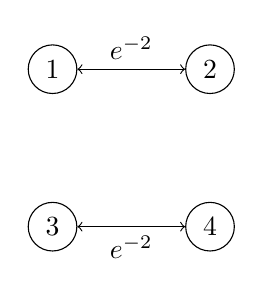
\begin{tikzpicture}
\begin{scope}[every node/.style={circle,draw}]
    \node (ul) at (0,2){1};
    \node (ur) at (2,2){2};
    \node (ll) at (0,0){3};
    \node (lr) at (2,0){4};
\end{scope}

    \path [<->] (ul) edge node[above]{$e^{-2}$} (ur);

    \path [<->] (ll) edge node[below]{$e^{-2}$} (lr);

\end{tikzpicture}

\end{enumerate}
\end{enumerate}

\newpage
\section{Classifying an Image using Grayscale Histograms}
\begin{enumerate}
\item Accuracy as a percentage of testing images classified correctly
\newline
$$ \frac{\text{Classified correctly}}{\text{Total test images}} = \frac{228}{350} \approx 65.1429\%  $$

\item One image correctly labeled as a car
\begin{figure}[h!]
    \subfloat[Histogram Image correctly labeled as a car]{\includegraphics[scale=1]{images/pos-8.png}}
\end{figure}

\item One image correctly labeled as not a car
\begin{figure}[h!]
    \subfloat[Histogram Image correctly labeled as not a car]{\includegraphics[scale=1]{images/neg-469.png}}
\end{figure}

\item One image incorrectly labeled as a car
\begin{figure}[h!]
    \subfloat[Histogram Image incorrectly labeled as a car]{\includegraphics[scale=1]{images/neg-195.png}}
\end{figure}

\item One image incorrectly labeled as not a car
\begin{figure}[h!]
    \subfloat[Histogram Image incorrectly labeled as not a car]{\includegraphics[scale=1]{images/pos-412.png}}
\end{figure}
\end{enumerate}

\newpage

\section{Classifying an Image using Gists}
\begin{enumerate}
\item Accuracy as a percentage of testing images classified correctly
\newline
$$ \frac{\text{Classified correctly}}{\text{Total test images}} = \frac{320}{350} \approx 91.4286\%  $$

\item One image correctly labeled as a car
\begin{figure}[h!]
    \subfloat[Histogram Image correctly labeled as a car]{\includegraphics[scale=1]{images/pos-412.png}}
\end{figure}

\item One image correctly labeled as not a car
\begin{figure}[h!]
    \subfloat[Histogram Image correctly labeled as not a car]{\includegraphics[scale=1]{images/neg-145.png}}
\end{figure}

\item One image incorrectly labeled as a car
\begin{figure}[h!]
    \subfloat[Histogram Image incorrectly labeled as a car]{\includegraphics[scale=1]{images/neg-195.png}}
\end{figure}

\item One image incorrectly labeled as not a car
\newline
My classification did not incorrectly label any image as not a car.
%\begin{figure}[h!]
%    \subfloat[Histogram Image incorrectly labeled as not a car]{\includegraphics[scale=1]{images/tmp.eps}}
%\end{figure}
\end{enumerate}

\end{document}
